\doublespacing % Do not change - required

\chapter{TIA Portal Program}

\thesisspacing % Do not change - required

In Chapter4, it was stated that a program was written in the TIA Portal software on PLCSim in order for the simulation environment created in the Factory IO environment to work correctly.
Here, the program written in the TIA Portal will be examined. As seen in Figures A1 and A2 below, the program consists of a total of 7 function blocks. Function blocks were preferred because the program does not look too complicated and is easier to examine and write.
\begin{figure}[H]
    \centering
    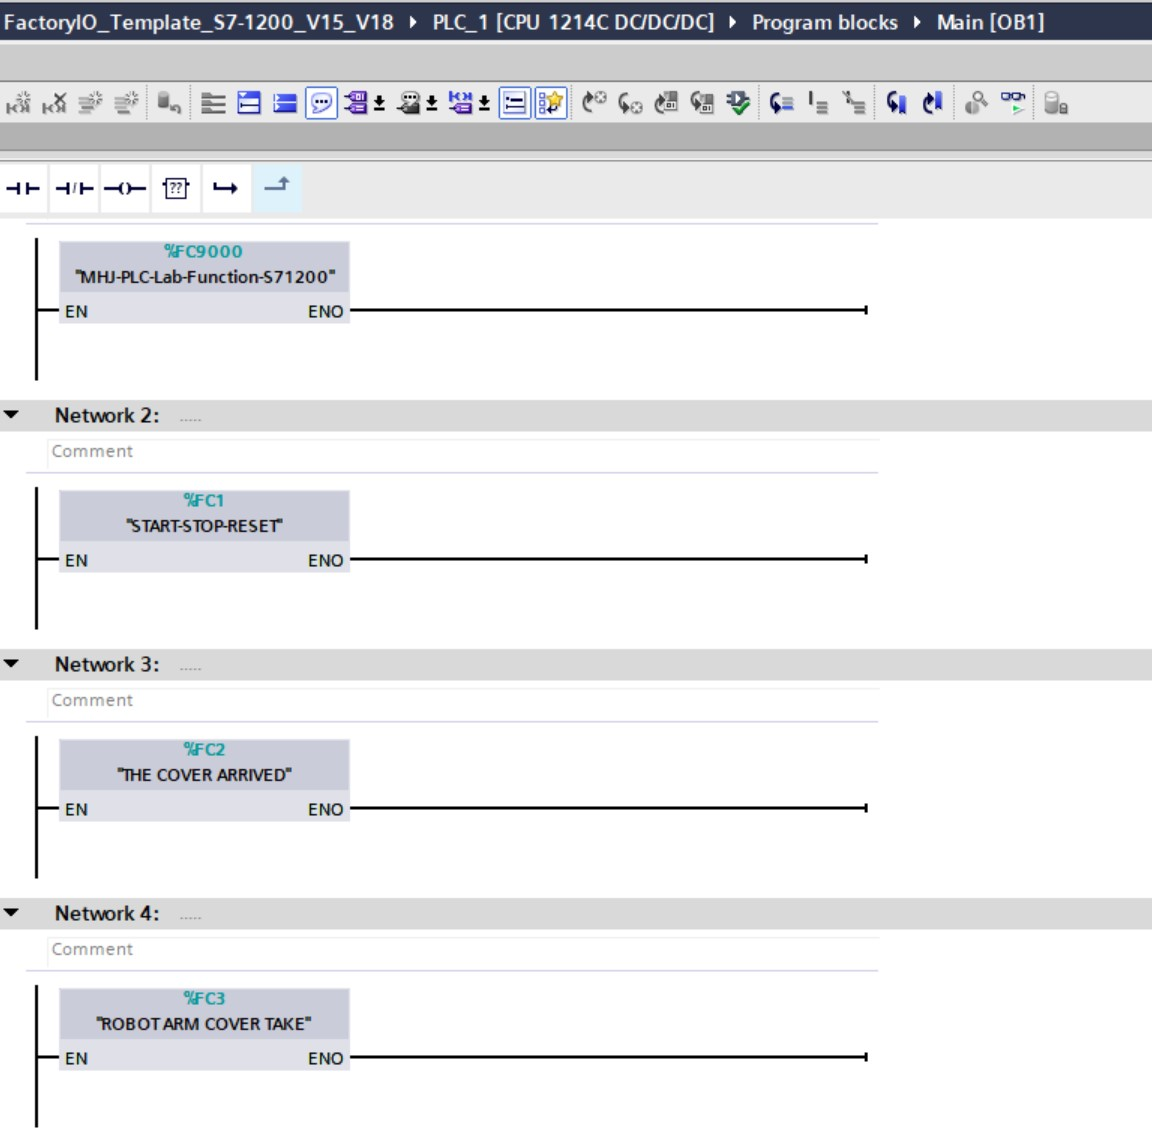
\includegraphics[width=0.70\columnwidth]{imgs/io/tia1.jpg}
    \caption[First four lines of the program]{First four lines of the program}
    \label{fig-magnitude}
\end{figure}%    
    \begin{figure}[H]
        \centering
        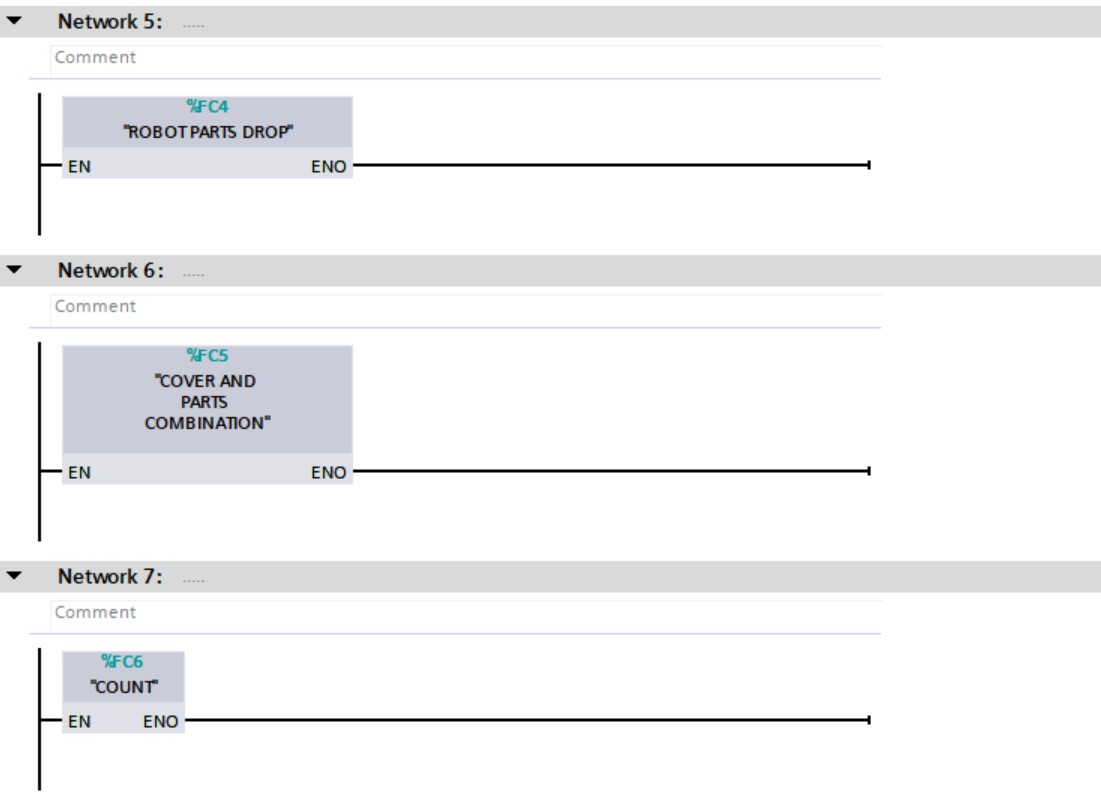
\includegraphics[width=0.70\columnwidth]{imgs/io/tia2.jpg}
        \caption[Last 3 lines of the program]{Last 3 lines of the program}
        \label{fig-magnitude}
    \end{figure}%
    Here, the first function block contains a ready-made function to establish the connection between TIA Portal and Factory IO. The internal structure of the block can be seen below.
\begin{figure}
    \centering
    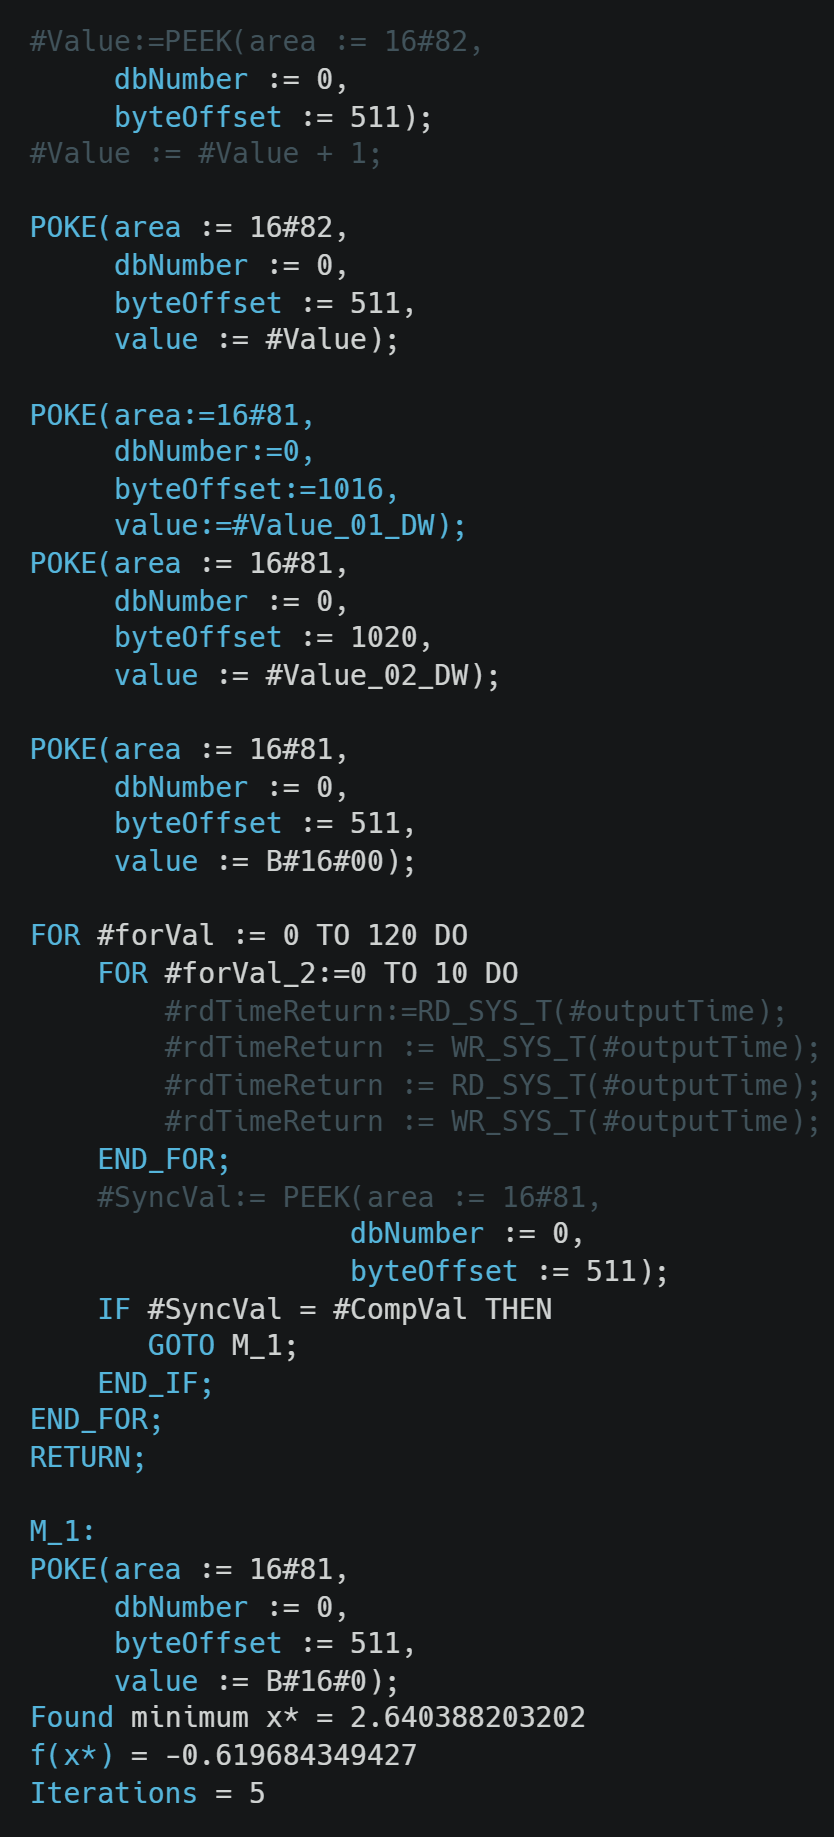
\includegraphics[width=0.50\columnwidth]{imgs/io/carbon.png}
    \caption[Function block 0]{Function block 0}
    \label{fig-magnitude}
\end{figure}%   

The function block seen in Figure A.4 above aims to start the system. Since the emergency stop button is normally connected to a closed contact in Factory IO, an open contact is connected here. Then, when the start button is pressed, the system starts.
\begin{figure}
    \centering
    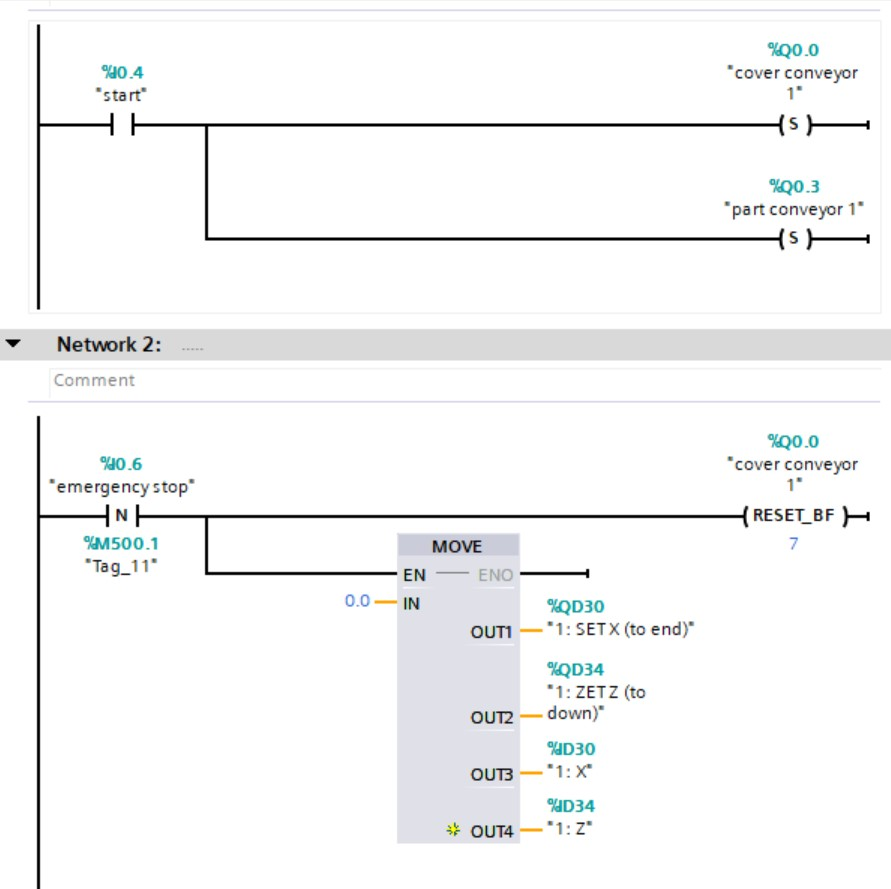
\includegraphics[width=0.60\columnwidth]{imgs/io/tia3.jpg}
    \caption[Function block 1]{Function block 1}
    \label{fig-magnitude}
\end{figure}%   


\begin{figure}[H]
    \centering
    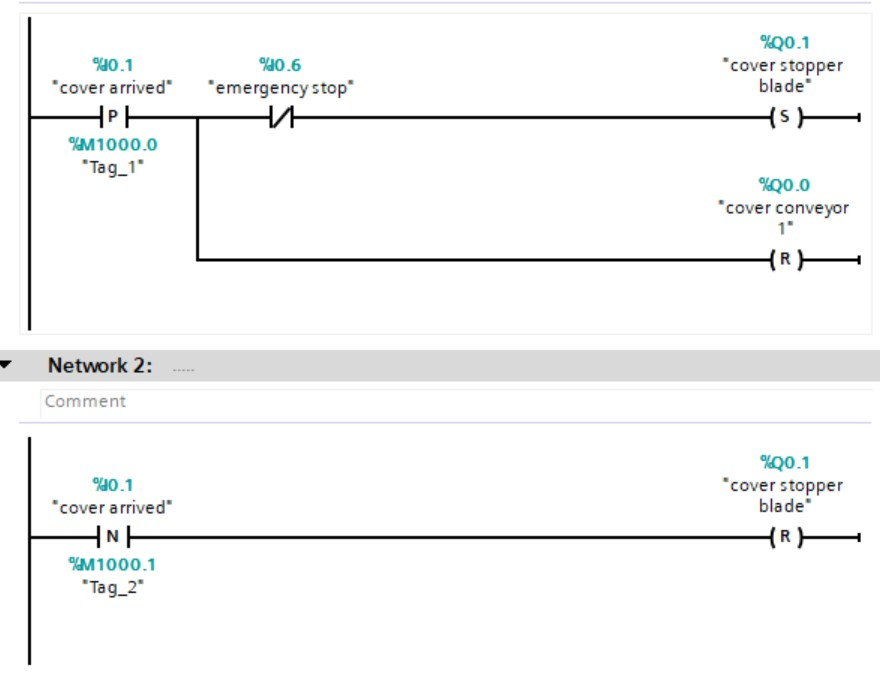
\includegraphics[width=0.60\columnwidth]{imgs/io/tia4.jpg}
    \caption[Function block 2]{Function block 2}
    \label{fig-magnitude}
\end{figure}% 
As seen in Figure A.5 above, when the sensor detecting the cover conveyor is active, the blade on the relevant side closes and the conveyor it comes to stops. When the sensor stops detecting, the blade opens again.

\begin{figure}[h!]
    \centering
    \begin{minipage}{0.45\textwidth}  
        \centering
        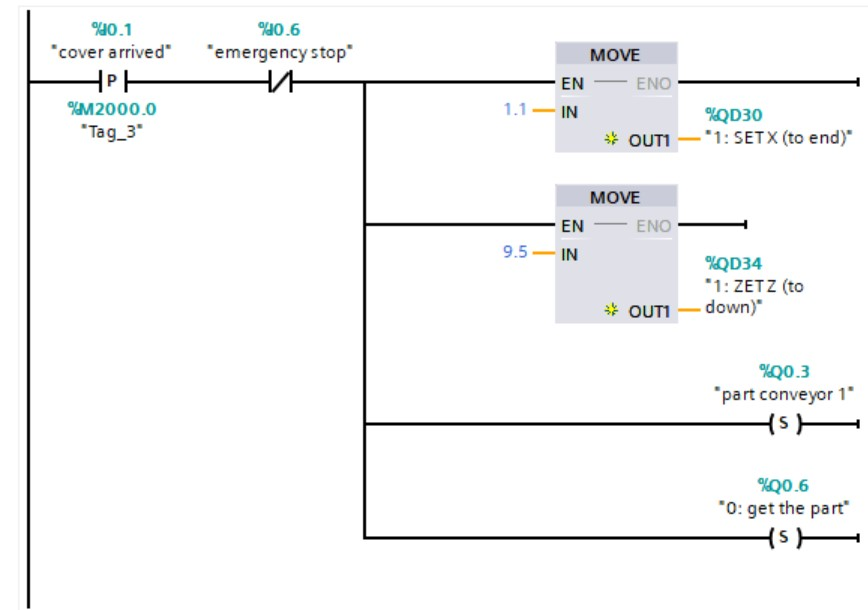
\includegraphics[width=\textwidth]{imgs/io/tia5.1.jpg}  
        \caption[Function blok 3 Network1]{Function blok 3 Network1}
        \label{fig:first}
    \end{minipage} \hfill  
    \begin{minipage}{0.45\textwidth}  
        \centering
        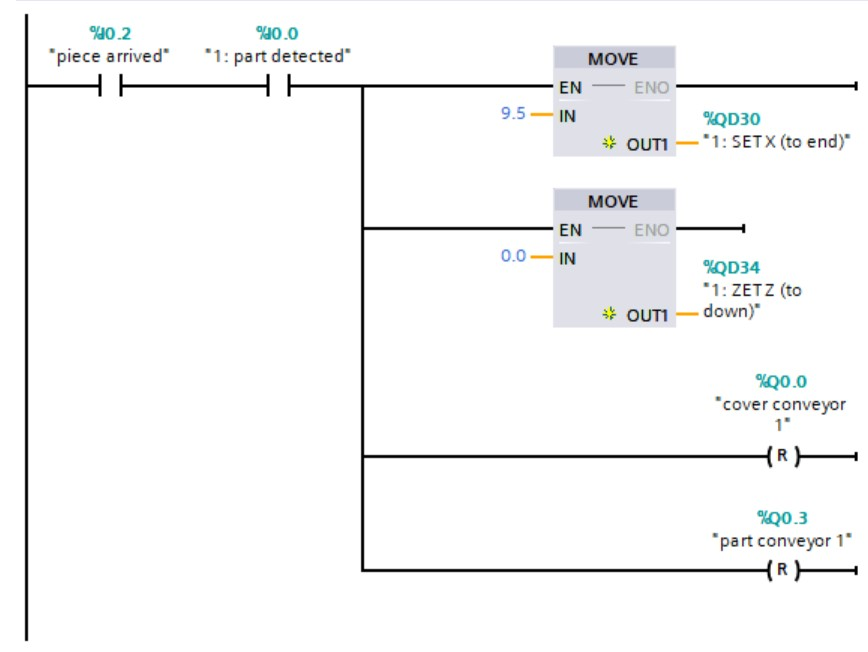
\includegraphics[width=\textwidth]{imgs/io/tia5.2.jpg}  
        \caption[Function blok 3 Network2]{Function blok 3 Network2}
        \label{fig:second}
    \end{minipage}
\end{figure}

In Figure A.6 above, after the lid is detected, the robot arm is provided with the help of a gripper to take the lid. These values ​​are provided to the x and z coordinates that were previously set by trial, that is, to be approximately on top of the lid.
In Figure A.7, the lid is taken to the determined coordinates and made ready to be combined with the part.

\begin{figure}[H]
    \centering
    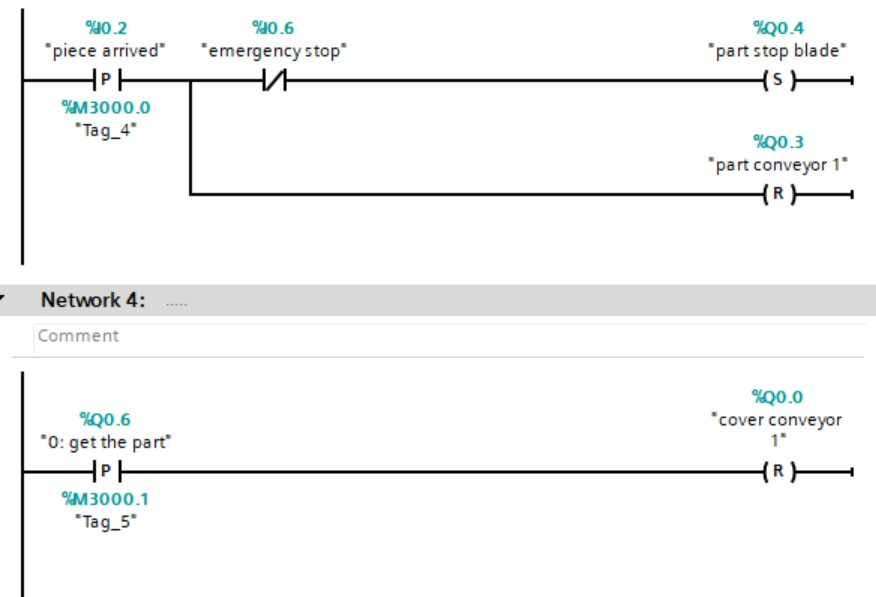
\includegraphics[width=0.60\columnwidth]{imgs/io/tia5.3.jpg}
    \caption[Function block 3 Network3 and Network4]{Function block 3 Network3 and Network4}
    \label{fig-magnitude}
\end{figure}% 

In Figure A.8 above, when the part sensor detects the object, the blade becomes active and the conveyor on which it stands goes into the off position. At the same time, after the gripper holds the lid, the lid conveyor stops accordingly.

\begin{figure}[H]
    \centering
    \begin{minipage}{0.45\textwidth}  
        \centering
        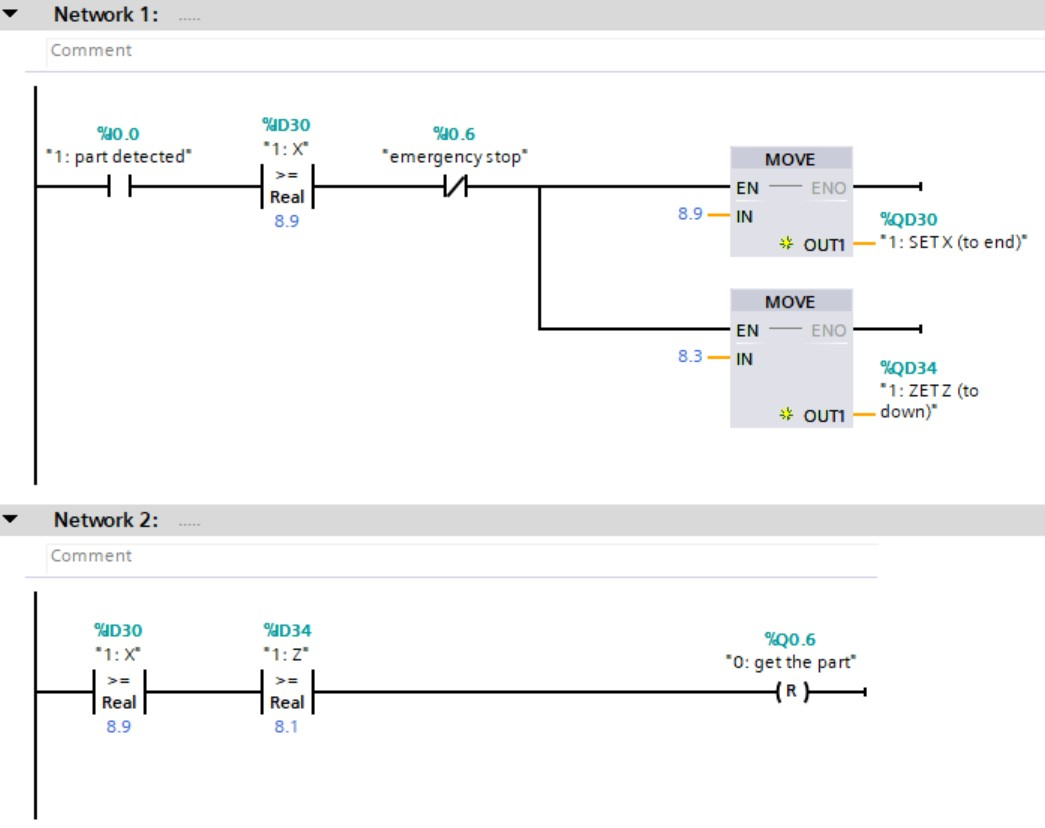
\includegraphics[width=\textwidth]{imgs/io/tia6.1.jpg}  
        \caption[Function blok 4 Network1 and Network2]{Function blok 4 Network1 and Network2}
        \label{fig:first}
    \end{minipage} \hfill  
    \begin{minipage}{0.45\textwidth}  
        \centering
        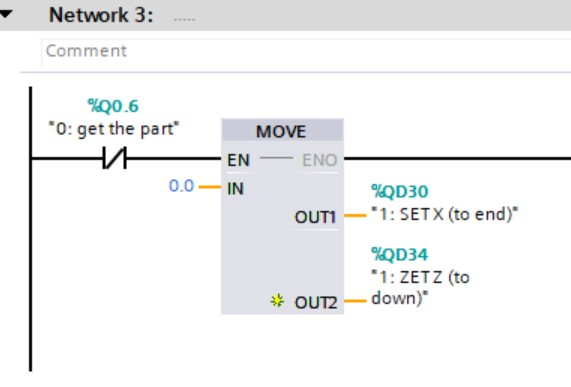
\includegraphics[width=\textwidth]{imgs/io/tia6.2.jpg} 
        \caption[Function blok 4 Network3]{Function blok 4 Network3}
        \label{fig:second}
    \end{minipage}
\end{figure}

In Figure A.9 above, when the robot arm reaches the desired position, it is assembled by dropping the cover onto the part.

In Figure A.10, the robot arm returns to the set starting position after releasing the lid.

\begin{figure}[H]
    \centering
    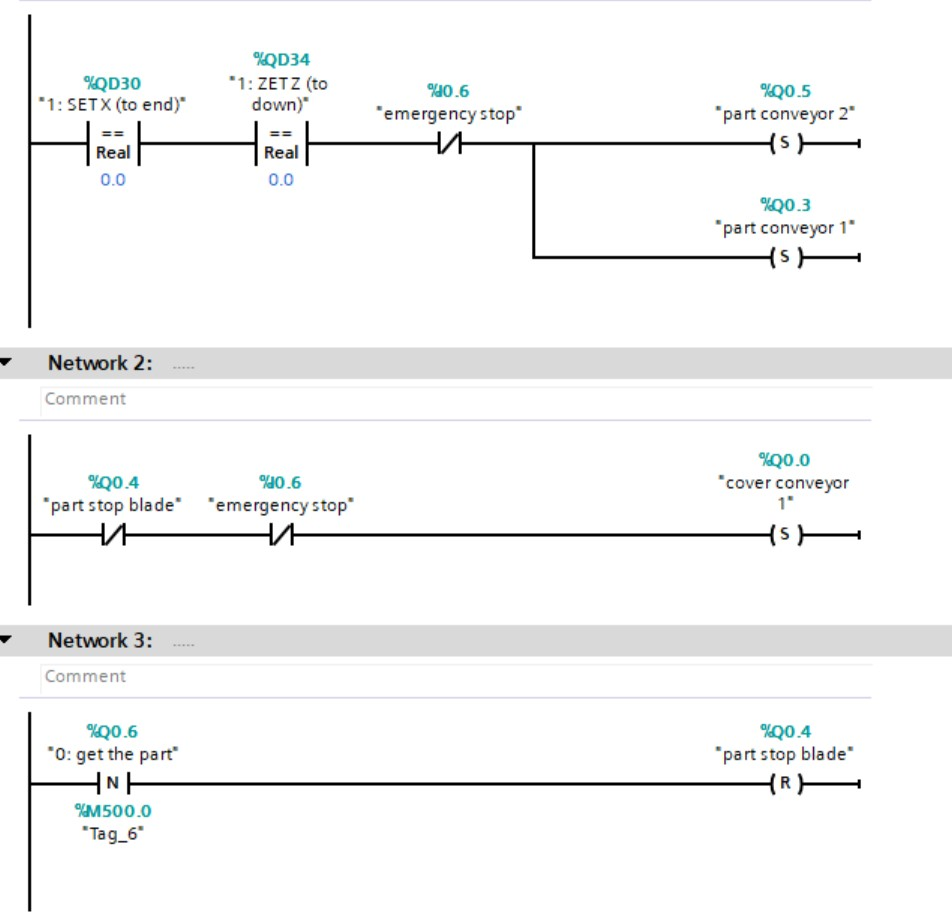
\includegraphics[width=0.60\columnwidth]{imgs/io/tia7.1.jpg}
    \caption[Function block 5 Network1 to Network3]{Function block 5 Network1 to Network3}
    \label{fig-magnitude}
\end{figure}% 

In Network 1 and Network 2 above, the conveyors are restarted. In Network 3, after the gripper releases the cover, the blade in front of the product is lifted. In this way, the product can move forward on the part conveyor.

\begin{figure}[H]
    \centering
    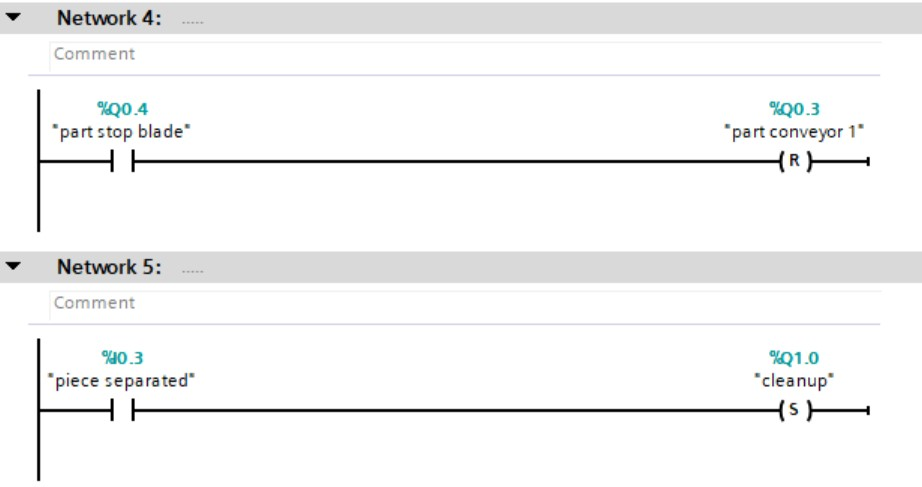
\includegraphics[width=0.60\columnwidth]{imgs/io/tia7.2.jpg}
    \caption[Function block 5 Network4 and Network5]{Function block 5 Network4 and Network5}
    \label{fig-magnitude}
\end{figure}% 

In Network 4 above, if the part blade is open, unnecessary operation of the 1st part conveyor is prevented. In this way, energy saving is achieved. In Network 5, after the created part passes the part separation sensor, the remover that cleans the created part at the end of the belt is activated.

\begin{figure}[H]
    \centering
    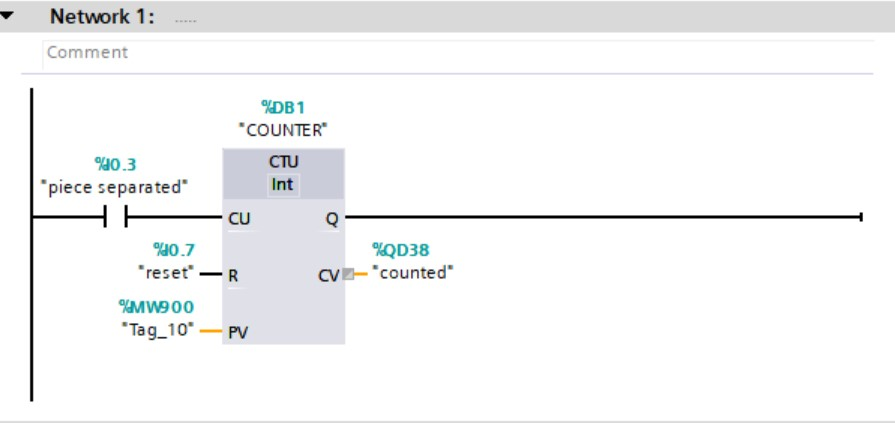
\includegraphics[width=0.60\columnwidth]{imgs/io/tia8.jpg}
    \caption[Function block 6]{Function block 6}
    \label{fig-magnitude}
\end{figure}% 
Here, a program part is seen where the products produced in the system are counted with an up counter block after the object created passes through the part separation sensor. A reset button is assigned to reset the counting process.

